\section{Technology}

When you start developing a piece of software of any kind, you have to pick a stack, that being: choosing which
technologies you're going to build your project on top of. This choice is probably the single most important decision of any
project (right after choosing what to build); getting this wrong can lead to headaches for months to come.

This project experienced two major rewrites where I swapped platform! The back-end, where the \textit{real calculations}
take place is written in "Go" (commonly referred to as Golang), for those who aren't familiar with it, it's like if
Python (Tygerjython) and C \footnote{The "C" programming language is the basis of most modern software infrastructure,
	being used by every operating system. It's very performant, however it has very few features, making the developer have
	to develop many things from scratch} had a baby; it has a simple syntax like python with 90\% of the performance of C.
The front-end (what the user actually sees) was originally written in HTML, CSS \& JavaScript using "Wails" to connect
the front- and back-ends. A few months into development I was experiencing too many issues with this setup: random
crashes, tight coupling \footnote{Coupling in software refers to how when one part of the software is changed, another
	related part also has to be as well. } and unexplainable bugs. This frustrated me to such an extent that I just stopped
working on the project for multiple weeks. Eventually I decided to completely rewrite the front-end in Godot, a free
game engine; the problem? I didn't know Godot. The smallest of changes required hours of reading the docs and struggling
around.

In the end I came back to my senses and tried developing the front-end in JavaScript, this time learning Web-Sockets . As any
developer knows, the 3rd time you write something is always better than the first two times. And so I stuck with this
right until the end.

\subsection{Implementation Details}

As with any software project, there are few things that go to plan and many lessons that were learnt along the way. One
of the key lessons I learnt during the  development of this project  is to avoid \textit{premature optimisation}.

\subsubsection*{Premature Optimisation}

\begin{quote}
	Premature optimization is the root of all evil (or at least most of it) in programming.

	\raggedleft{\textbf{Donald Knuth}}
\end{quote}

Premature optimisation is the act of devoting a significant amount of optimising for task you might not truly need to
optimise for.

A funny example of this was while developing budget mode. In budget mode the player is able to see the predicted outcome
of the decisions they are about to make. To be able to clearly differentiate between budget mode and normal mode, I
wanted the colour scheme to change such that instead of blue being the primary colour, green was.

\begin{figure}[h]
	\centering
	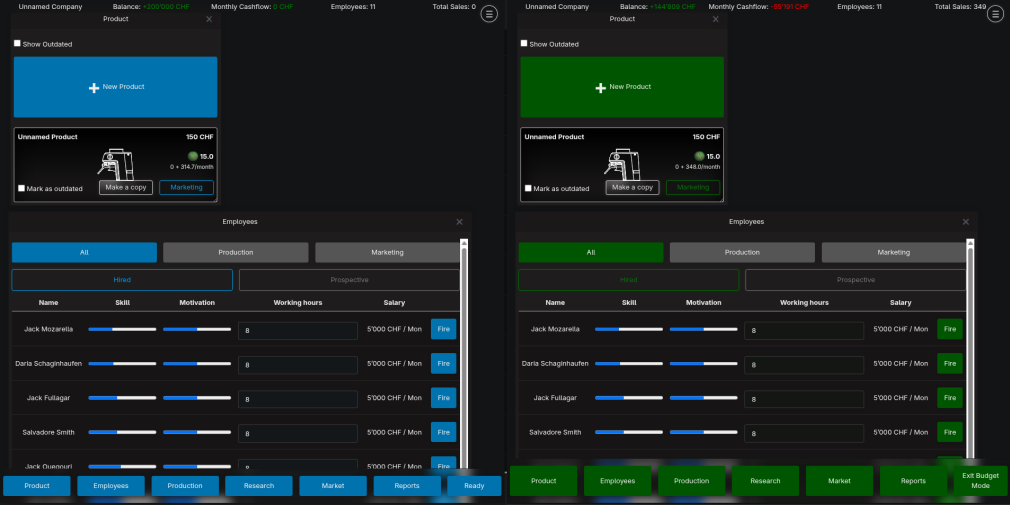
\includegraphics[width=0.9\textwidth]{assets/interface_combined.png}
	\caption{What I wanted to achieve}
\end{figure}

Having heard of relative colours using the CSS\footnote{CSS is the technology used to style websites and web apps.
	CSS files are also referred to as style sheets.} \verb|color()| and \verb|color-mix| functions I wanted to adapt my
current style sheet to use these relative colours. I just had one problem: the style sheet I was using was multiple
hundreds of lines long (quite long!) and I didn't want to manually edit all of that! So what is the logical answer to
this predicament? Is it to just make a new style sheet that approximated the previous one except that it had these
relative colours, given that I was using a very small subset of the features of the style sheet? NO! The answer is to
write a small program that reads, parses and extracts colours from a CSS file, converts the colours to relative colours
(if possible) and finally rewrites the new CSS file. This, in fact, was not the most logical solution. It is not only
unnecessarily trying to automate a task that realistically takes a half hour, but it also steps into the
\textit{extremely complex}\footnote{For more info on digital colours see: "Everything About Color in 25 Minutes" by Juxtopposed.
	\href{https://www.youtube.com/watch?v=srRI7yMjGz0\&t=6s}{https://www.youtube.com/watch?v=srRI7yMjGz0\&t=6s}} domain of digital colours,
a domain that I had almost no knowledge in.

I ended up wasting a week of time calculating and coding this "simple" app to convert colours. The maths to derive the
relative components of a colour already took multiple pages and the program itself was hundreds of lines long. This
misadventure thoroughly taught me not to try to prematurely optimise something that, in the end, I didn't even need.
